% ==========================================
% Section 7: Unsupported Data Types (Slides 24-29)
% ==========================================

% Slide 24: Unsupported Data Types
\begin{frame}{انواع داده‌های پشتیبانی‌نشده}
\begin{itemize}
  \item \textbf{همه الگوریتم‌های یادگیری از تمام انواع داده پشتیبانی نمی‌کنند:}
  \begin{itemize}
    \item برخی الگوریتم‌ها (مانند \lr{SVM} و شبکه‌های عصبی) قادر به پردازش مستقیم ویژگی‌های دسته‌ای/متنی نیستند و فقط بردار عددی می‌پذیرند.
    \item برخی دیگر (مانند \lr{Naive Bayes} استاندارد) تنها با مقادیر دسته‌ای یا گسسته به خوبی کار می‌کنند.
  \end{itemize}
  \vspace{0.3cm}
  \item \textbf{انواع داده‌های متداول نیازمند تبدیل:}
  \begin{itemize}
    \item متغیرهای دسته‌ای و کیفی (\lr{Categorical Attributes})
    \item متغیرهای عددی نیازمند گسسته‌سازی (\lr{Discretization})
    \item داده‌های تاریخ و زمان (\lr{Date \& Time})
    \item متون آزاد و اسناد (\lr{Textual Data})
  \end{itemize}
\end{itemize}
\end{frame}

% Slide 25: Ordinal Encoding
\begin{frame}{تبدیل ویژگی‌های دسته‌ای به عددی: ویژگی‌های ترتیبی}
\begin{itemize}
  \item \textbf{ویژگی‌های ترتیبی (\lr{Ordinal Attributes})}
  \begin{itemize}
    \item ترتیب و توالی میان مقادیر دارای بار مفهومی است (مانند \lr{Grade = A, A-, B+, B, B-, C+, C, C-}).
    \item نگاشت متناظر به مقادیر عددی با حفظ ترتیب: \lr{A=8, A-=7, B+=6, B=5, B-=4, C+=3, C=2, C-=1}
  \end{itemize}
\end{itemize}
\vspace{0.15cm}
\centering
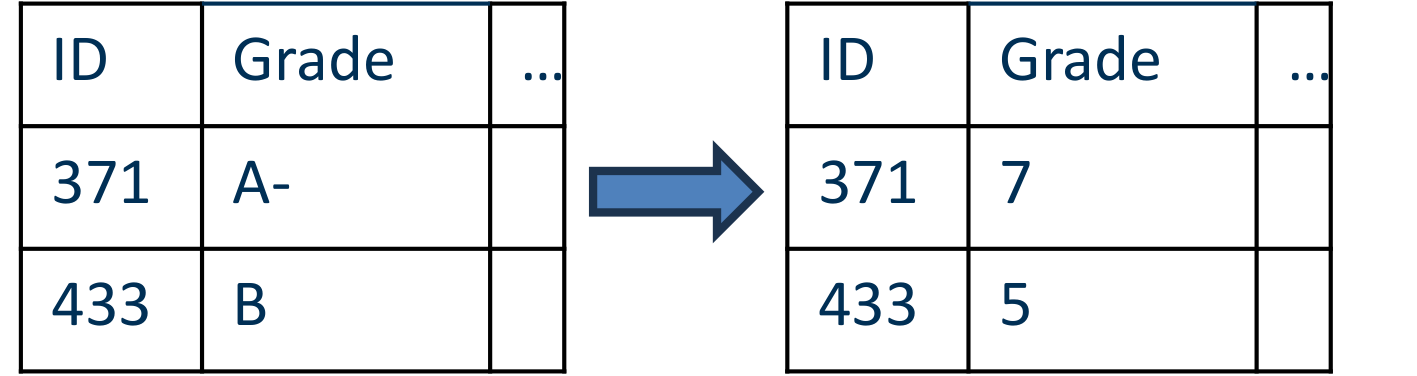
\includegraphics[width=0.62\textwidth]{images/page_25_table.png}
\vspace{0.2cm}
\begin{itemize}
  \item استفاده از چنین کدگذاری‌ای به مدل اجازه یادگیری قواعد معنادار را می‌دهد (مثلاً \lr{grade > 6 $\to$ excellent\_student = true}).
  \item \textbf{پیاده‌سازی در پایتون:} \codebox{OrdinalEncoder}
\end{itemize}
\end{frame}

% Slide 26: One-Hot Encoding
\begin{frame}{تبدیل ویژگی‌های دسته‌ای به عددی: ویژگی‌های اسمی}{\lr{Conversion: Categorical to Numeric}}
\begin{itemize}\setlength{\itemsep}{2pt}
  \item \textbf{ویژگی‌های اسمی و بدون ترتیب (\lr{Nominal Attributes}):}
  \begin{itemize}\setlength{\itemsep}{1pt}
    \item \textbf{کدگذاری یکتا (\lr{One-Hot Encoding}):} برای هر مقدار $v$ یک متغیر پرچم دودویی $C_v$ ایجاد می‌شود که در صورت برابری ۱ و در غیر این صورت ۰ است.
  \end{itemize}
\end{itemize}
\vspace{0.1cm}
\centering
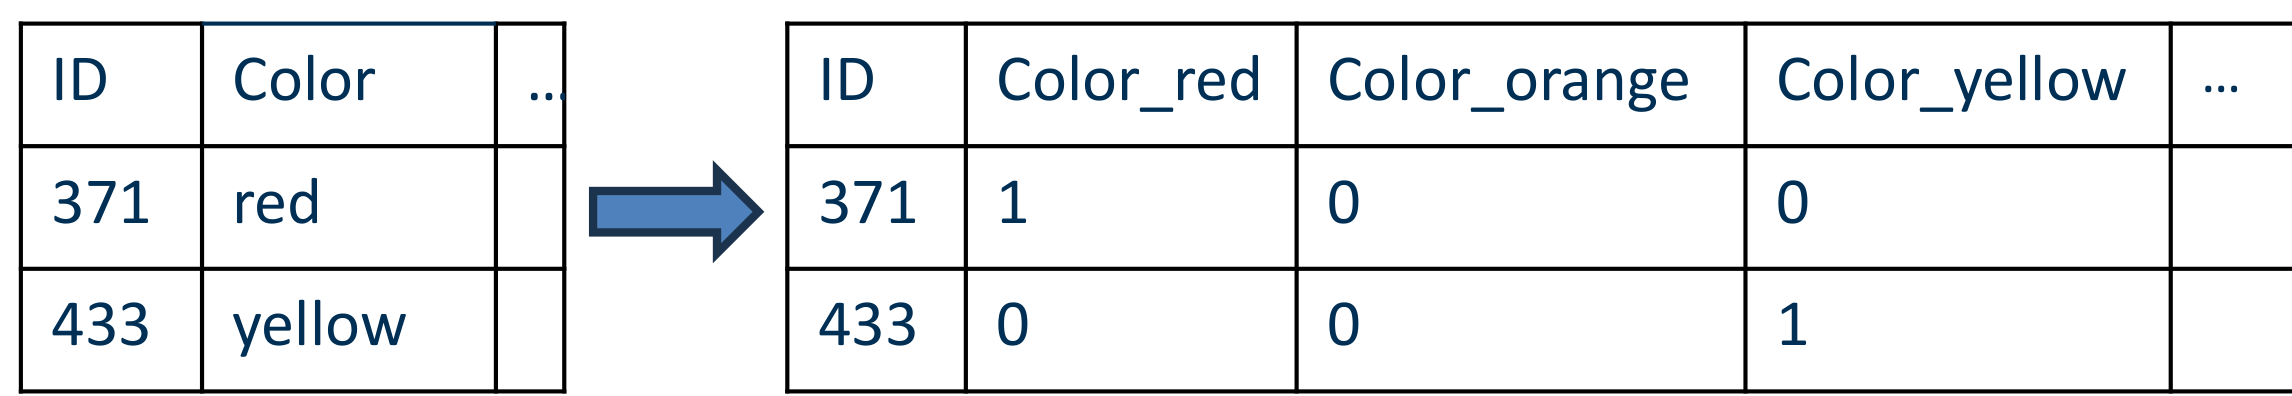
\includegraphics[width=0.78\textwidth]{images/page_26_table.png}
\vspace{0.15cm}
\begin{itemize}\setlength{\itemsep}{2pt}
  \item \textbf{پیاده‌سازی در پایتون:} \codebox{OneHotEncoder}
  \item \textbf{حالت خاص -- ویژگی‌های دودویی (\lr{Binary}):} مانند \lr{student = yes, no}
  \begin{itemize}\setlength{\itemsep}{1pt}
    \item برای \lr{Student = yes $\to$ student\_binary = 0}
    \item برای \lr{Student = no $\to$ student\_binary = 1}
  \end{itemize}
\end{itemize}
\end{frame}

% Slide 27: High Cardinality
\begin{frame}{تبدیل ویژگی‌های دسته‌ای با مقادیر پرشمار}
\begin{columns}[c]
  \begin{column}{0.55\textwidth}
    \begin{itemize}
      \item \textbf{مقادیر متعدد (\lr{Many Values}):}
      \begin{itemize}
        \item کد ایالت‌های آمریکا (\lr{50} مقدار)
        \item کد شغل (\lr{7,000} مقدار، اما تنها چند مقدار پرتکرار)
      \end{itemize}
      \vspace{0.2cm}
      \item \textbf{رویکردها:}
      \begin{itemize}
        \item دستی، با دانش زمینه (مثلاً گروه‌بندی ایالت‌ها)
        \item استفاده از ویژگی‌های دودویی و سپس اعمال کاهش بعد
      \end{itemize}
    \end{itemize}
  \end{column}
  \begin{column}{0.43\textwidth}
    \centering
    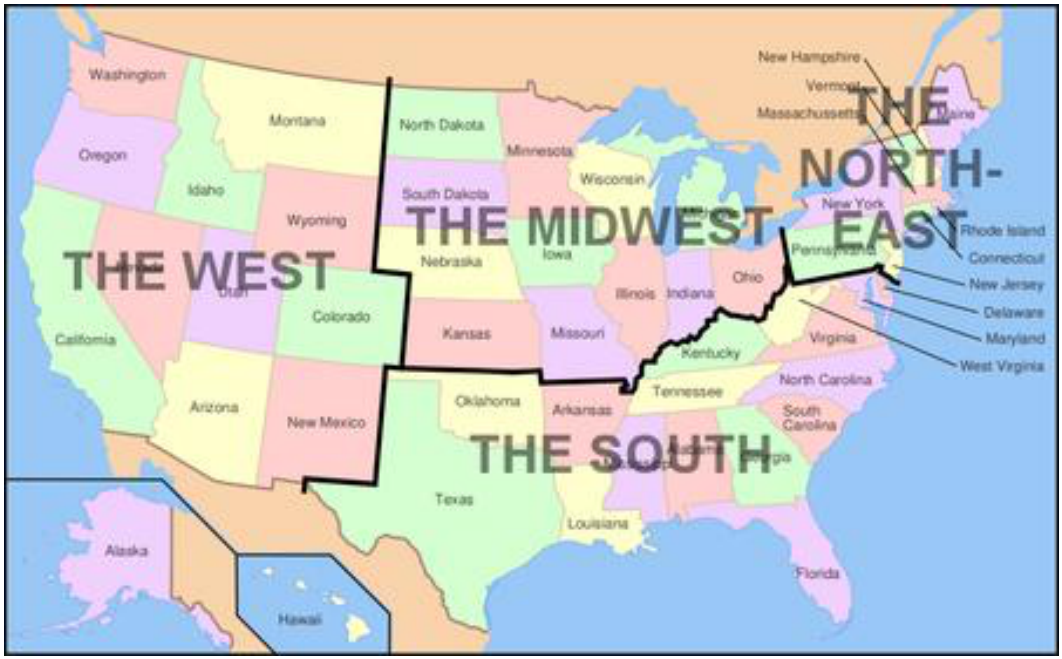
\includegraphics[width=\textwidth]{images/page_27_img_1.png}
  \end{column}
\end{columns}
\end{frame}

% Slide 28: Numeric to Ordinal / Discretization
\begin{frame}{تبدیل مقادیر عددی به ترتیبی (گسسته‌سازی)}
\begin{itemize}
  \item \textbf{یادآوری: گسسته‌سازی برای درخت تصمیم (\lr{Discretization})}
  \begin{itemize}
    \item مقادیر ویژگی (مثلاً سن افراد): $\{0, 4, 12, 16, 16, 18, 24, 26, 28\}$
  \end{itemize}
  \vspace{0.2cm}
  \item \textbf{گسسته‌سازی با بازه‌های هم‌اندازه (\lr{Equal-interval binning})} -- مثلاً برای پهنای بازه ۱۰:
  \begin{itemize}
    \item بازه ۱: $0, 4$ \hfill $[-\infty, 10)$
    \item بازه ۲: $12, 16, 16, 18$ \hfill $[10, 20)$
    \item بازه ۳: $24, 26, 28$ \hfill $[20, +\infty)$
  \end{itemize}
  \vspace{0.2cm}
  \item \textbf{گسسته‌سازی با بسامد یکسان (\lr{Equal-frequency binning})} -- مثلاً برای تراکم ۳ نمونه در هر بازه:
  \begin{itemize}
    \item بازه ۱: $0, 4, 12$ \hfill $[-\infty, 14)$
    \item بازه ۲: $16, 16, 18$ \hfill $[14, 21)$
    \item بازه ۳: $24, 26, 28$ \hfill $[21, +\infty)$
  \end{itemize}
\end{itemize}
\end{frame}

% Slide 29: Dates and Times
\begin{frame}{مدیریت ویژگی‌های تاریخ و زمان}
\begin{itemize}
  \item \textbf{تاریخ‌ها و زمان‌ها با فرمت‌های گوناگون ثبت می‌شوند:}
  \begin{itemize}
    \item گام نخست: استانداردسازی و تجزیه متن تاریخ (\lr{Normalize \& Parse})
  \end{itemize}
  \vspace{0.2cm}
  \item \textbf{تاریخ‌ها حامل اطلاعات جذاب و فراوانی هستند:}
  \begin{itemize}
    \item مثال: تحلیل رفتار خرید مشتریان
    \item زمان در طول روز (\lr{Time of day})
    \item روز کاری در برابر تعطیلات آخر هفته (\lr{Weekday vs. Weekend})
    \item ابتدا در برابر انتهای ماه (\lr{Begin vs. End of month})
    \item خود ماه، فصل و فصل سال (\lr{Month, Quarter, Season})
  \end{itemize}
  \vspace{0.2cm}
  \item \textbf{پایتون:} استفاده از کتابخانه \lr{datetime}
\end{itemize}
\end{frame}
